\documentclass{article}
\usepackage[margin=1in]{geometry}
\usepackage{amsmath}
\usepackage{amssymb}
\usepackage{amsthm}
\usepackage{bm}
\usepackage{hyperref}
\usepackage{graphicx}
\usepackage{caption}
\usepackage{listings}
\usepackage{xcolor}
\usepackage{float}
\usepackage{placeins}
\graphicspath{{figures/}}

% Code style
\lstdefinestyle{code}{
  basicstyle=\ttfamily\small,
  numbers=left,
  numberstyle=\tiny,
  numbersep=8pt,
  keywordstyle=\color{blue},
  commentstyle=\color{teal!70!black},
  stringstyle=\color{orange!70!black},
  showstringspaces=false,
  breaklines=true,
  frame=single,
  framerule=0.3pt,
  rulecolor=\color{black!15}
}
\lstset{style=code}

\title{Model Training and Parameter Adjustment Strategies}
\author{}
\date{\today}

\begin{document}
\maketitle
\tableofcontents
\FloatBarrier

\section{Hyperparameter Selection: Batch Size, Learning Rate, and Optimizer}
Hyperparameters govern the optimization landscape and generalization performance. Good defaults narrow the search space, while principled scaling rules enable efficient exploration on new hardware budgets. Figure~\ref{fig:hyperparameter_landscape} visualizes typical interactions among learning rate, batch size, and optimizer choice.

\subsection{Batch Size}
Batch size $B$ trades statistical efficiency for hardware utilization. The gradient noise scale $\mathcal{G}$ captures how stochasticity changes with $B$:
\begin{equation}
  \mathcal{G} = \frac{\mathbb{E}\bigl[\|\nabla \mathcal{L}(\boldsymbol{\theta}; \mathcal{B})\|_2^2\bigr] - \|\nabla \mathcal{L}(\boldsymbol{\theta})\|_2^2}{\|\nabla \mathcal{L}(\boldsymbol{\theta})\|_2^2}.
\end{equation}
When $B \gg \mathcal{G}$, the variance reduction saturates and larger batches offer diminishing returns. Practically, one scales $B$ to match available memory and uses gradient accumulation to emulate large batches under small-memory constraints.

\subsection{Learning Rate Policies}
The ``linear scaling rule'' suggests $\eta \approx \eta_0 \cdot B / B_0$ when increasing batch size $B$. However, stability requires warm-up to prevent divergence:
\begin{equation}
  \eta_t =
  \begin{cases}
    \eta_{\text{target}} \frac{t}{T_w}, & 0 \le t \le T_w, \\
    \eta_{\text{schedule}}(t - T_w), & t > T_w.
  \end{cases}
\end{equation}
Adaptive schedules---cosine annealing, inverse square-root decay, or cyclical policies---balance rapid progress with fine convergence. Learning rate range tests sweep $\eta$ across orders of magnitude to identify a stability window.

\subsection{Optimizer Selection}
The optimizer defines how gradients translate into parameter updates. Key families include:
\begin{itemize}
  \item \textbf{SGD with momentum:} Suited for large-scale vision tasks; the update $\mathbf{v}_{t+1} = \mu \mathbf{v}_{t} + \nabla_{\boldsymbol{\theta}} \mathcal{L}_t$ and $\boldsymbol{\theta}_{t+1} = \boldsymbol{\theta}_t - \eta \mathbf{v}_{t+1}$ damps oscillations along ravines.
  \item \textbf{AdamW:} Maintains per-parameter adaptive learning rates via moment tracking while decoupling weight decay. Typically excels on language models and sparse gradients.
  \item \textbf{Lion, LAMB, Adafactor:} Designed for transformer-scale models with hardware-aware modifications (e.g., layer-wise scaling, reduced memory footprint).
\end{itemize}
Mixed-precision training interacts with optimizer choice because dynamic loss scaling can skew moment estimation. Ensuring gradient clipping precedes optimizer updates avoids exploding updates in low-precision regimes.

\subsection{Search Strategies}
Random search and Bayesian optimization remain strong baselines for hyperparameter tuning. Define a search space $\mathcal{S}$ with log-uniform priors for scale-sensitive parameters (e.g., $\log_{10} \eta \sim U[-5, -1]$). Successive halving and population-based training allocate more resources to promising configurations. The following snippet demonstrates a simple random search loop:

\begin{lstlisting}[language=Python, caption={Random search over batch size, learning rate, and optimizer family.}]
import random
from itertools import count

search_space = {
    "batch_size": [64, 128, 256, 512],
    "lr": lambda: 10 ** random.uniform(-4.5, -2.5),
    "optimizer": lambda: random.choice(["sgd_momentum", "adamw", "lion"]),
}

def sample_config():
    return {
        "batch_size": random.choice(search_space["batch_size"]),
        "lr": search_space["lr"](),
        "optimizer": search_space["optimizer"](),
    }

best = None
for trial in count(start=1):
    cfg = sample_config()
    metrics = train_and_evaluate(cfg)  # user-defined
    if best is None or metrics["val_accuracy"] > best["val_accuracy"]:
        best = {"trial": trial, **cfg, **metrics}
    if stopping_criterion(best, trial):
        break

print(f"Best config: {best}")
\end{lstlisting}

\begin{figure}[H]
  \centering
  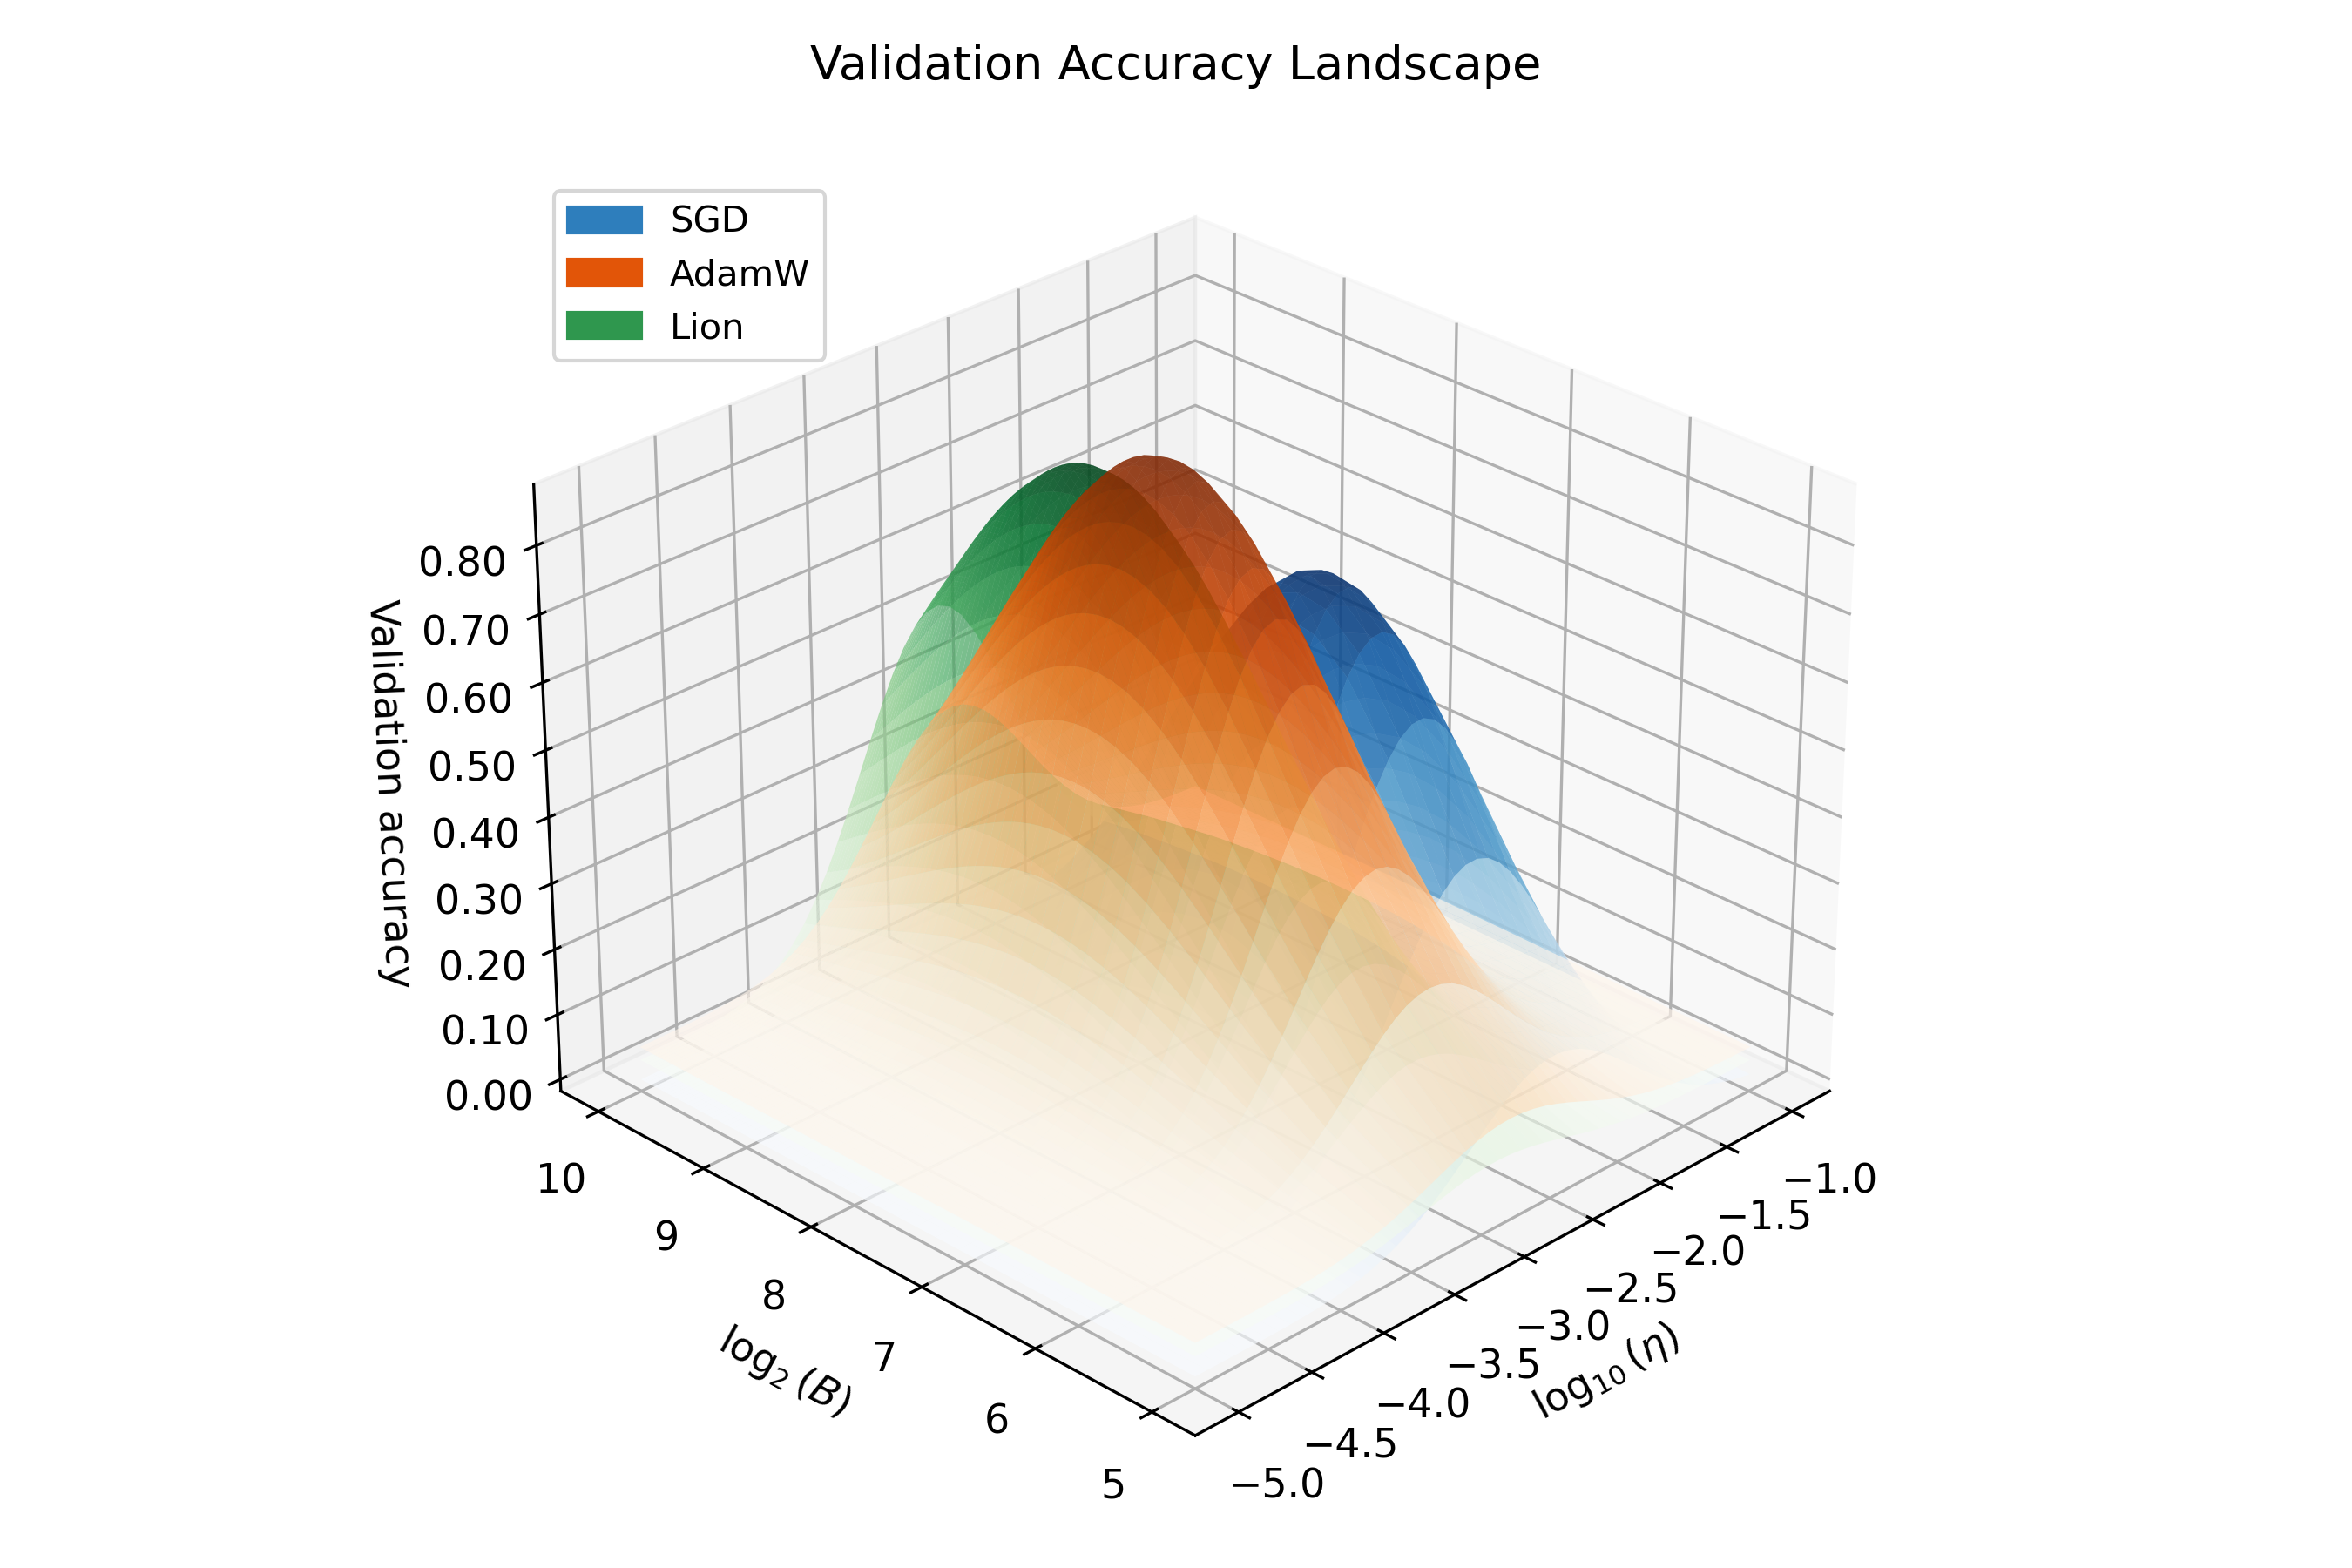
\includegraphics[width=0.85\textwidth]{hyperparameter_landscape.png}
  \caption{Validation performance as a function of learning rate, batch size, and optimizer choice. The front surface highlights configurations that balance speed and generalization.}
  \label{fig:hyperparameter_landscape}
\end{figure}
\FloatBarrier

\section{Early Stopping and Checkpointing}
Early stopping monitors a validation metric to halt training when overfitting emerges. Checkpointing persists model states for recovery, ensemble averaging, or fine-tuning. Figure~\ref{fig:early_stopping_checkpoint} summarizes typical dynamics.

\subsection{Patience-Based Early Stopping}
Given validation metric $m_t$, patience $p$, and minimal improvement threshold $\delta$, stop at step $t^\star$ if
\begin{equation}
  t^\star = \min \left\{ t : \max_{t - p \le k \le t} m_k \le m_{t-p} + \delta \right\}.
\end{equation}
Restoring the best checkpoint avoids discarding late-stage improvements. Smoothing via exponential moving averages reduces spurious triggers caused by noisy validation data.

\subsection{Checkpoint Policies}
Checkpoint frequency trades storage for robustness. Common options include:
\begin{itemize}
  \item \textbf{Rolling windows:} Maintain the latest $K$ checkpoints and prune older ones.
  \item \textbf{Best-$N$:} Store top-performing snapshots for later ensemble averaging.
  \item \textbf{Event-driven:} Trigger on metric improvements exceeding $\delta$ or milestones (e.g., every doubling of epochs).
\end{itemize}
Storing optimizer states (momenta, variance estimates) is essential for resuming training faithfully. For large models, sharded checkpoint formats (e.g., PyTorch FSDP or TensorFlow Checkpoint shards) decompose tensors to reduce per-node memory pressure.

\subsection{Integration with Hyperparameter Search}
When running asynchronous hyperparameter search, early stopping accelerates exploration by terminating underperforming trials. Population-based training periodically replaces bad configurations with perturbed copies of top performers, necessitating lightweight checkpoints to reduce latency.

\subsection{Sample Implementation}

\begin{lstlisting}[language=Python, caption={Early stopping with checkpoint rotation using PyTorch.}]
import torch
from pathlib import Path

def save_checkpoint(path: Path, model, optimizer, step: int, metrics: dict):
    state = {
        "model": model.state_dict(),
        "optimizer": optimizer.state_dict(),
        "step": step,
        "metrics": metrics,
    }
    torch.save(state, path)

def early_stopping_loop(dataloader, model, optimizer, scheduler, patience=10, min_delta=1e-4):
    best_metric = -float("inf")
    best_path = Path("checkpoints/best.pt")
    wait = 0
    for step, batch in enumerate(dataloader, start=1):
        train_step(model, optimizer, batch)
        if step % 100 == 0:
            metric = evaluate_validation(model)
            scheduler.step(metric)
            save_checkpoint(Path(f"checkpoints/step_{step}.pt"), model, optimizer, step, {"val": metric})
            rotate_checkpoints(Path("checkpoints"), keep=3)
            if metric > best_metric + min_delta:
                best_metric = metric
                wait = 0
                save_checkpoint(best_path, model, optimizer, step, {"val": metric})
            else:
                wait += 1
                if wait >= patience:
                    restore_checkpoint(best_path, model, optimizer)
                    print(f"Early stop at step {step} with best metric {best_metric:.4f}")
                    break
\end{lstlisting}

\begin{figure}[H]
  \centering
  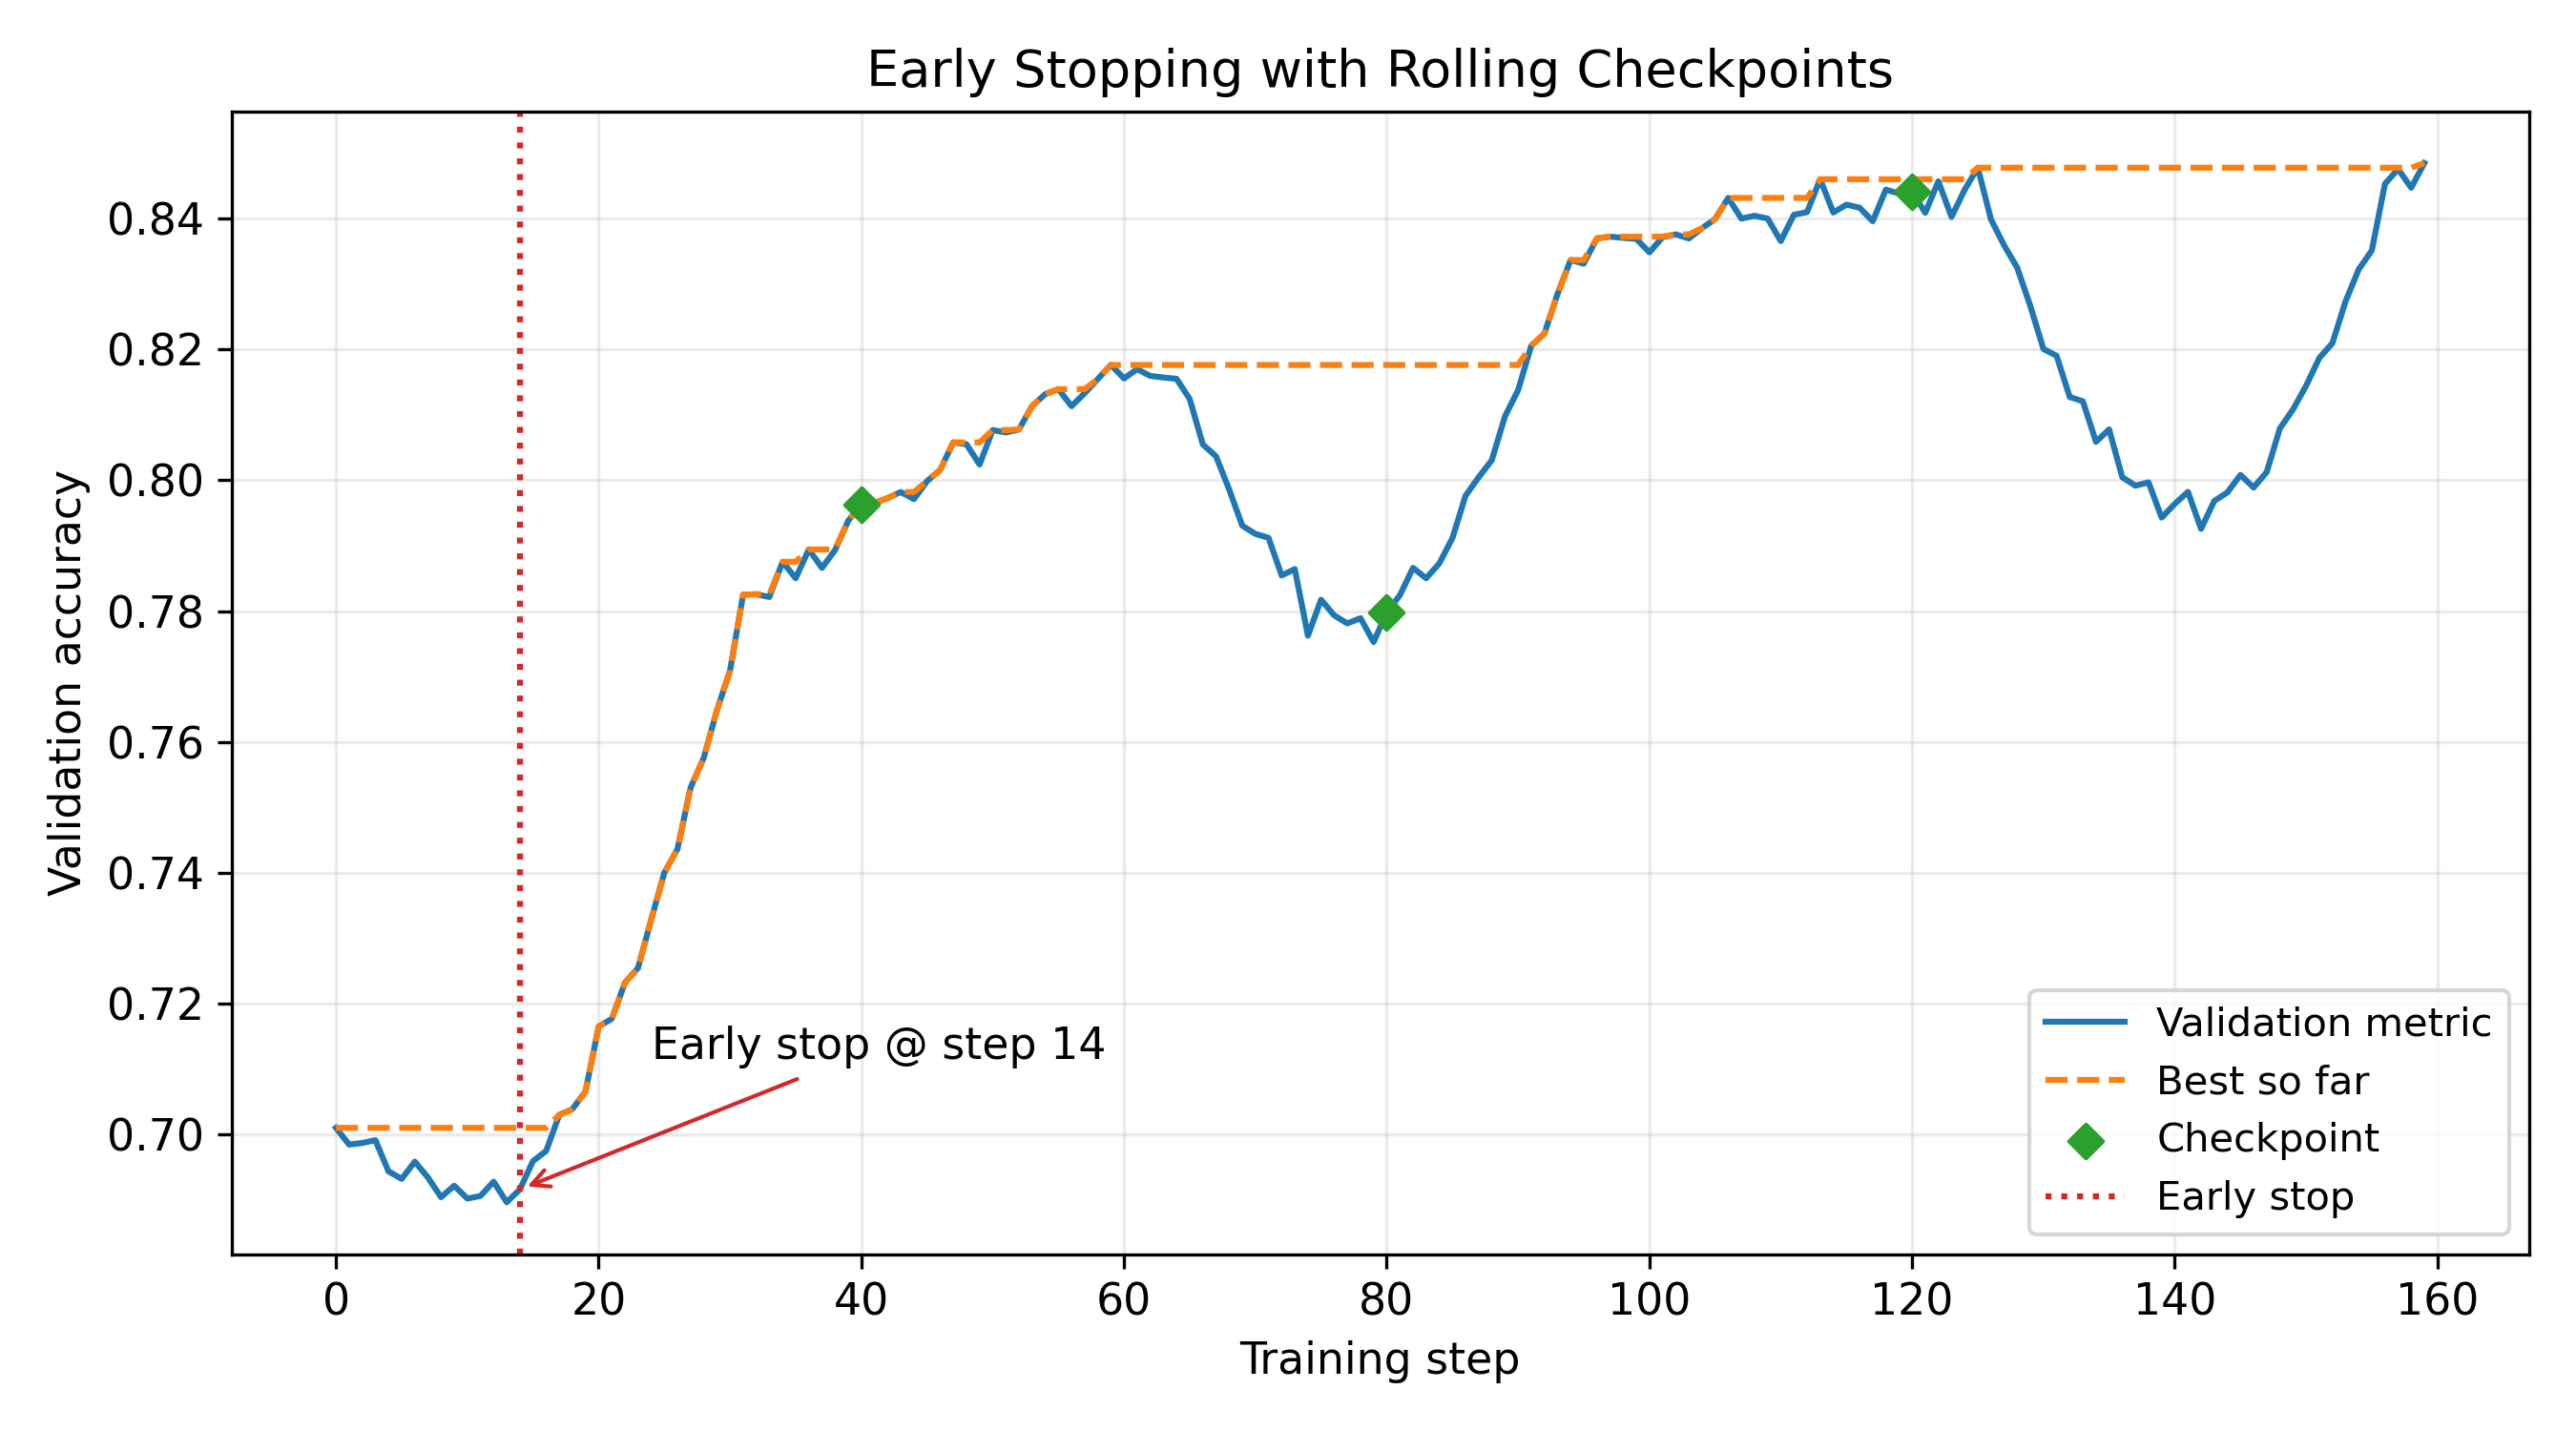
\includegraphics[width=0.85\textwidth]{early_stopping_checkpoint.png}
  \caption{Validation metric evolution with early stopping. The best checkpoint occurs before overfitting; subsequent checkpoints enable ensembling or warm restarts.}
  \label{fig:early_stopping_checkpoint}
\end{figure}
\FloatBarrier

\section{Large-Scale and Distributed Training}
Modern models require distributed computation across accelerators and nodes. Distributed training strategies balance communication overhead with parallel efficiency. Figure~\ref{fig:distributed_training_topologies} compares prevalent topologies, while Figure~\ref{fig:scaling_efficiency} illustrates scaling behavior.

\subsection{Data Parallelism}
Data parallelism replicates model parameters across $N$ workers, each processing disjoint mini-batches. Gradients are aggregated via all-reduce:
\begin{equation}
  \boldsymbol{\theta}_{t+1} = \boldsymbol{\theta}_t - \eta \frac{1}{N} \sum_{n=1}^{N} \nabla_{\boldsymbol{\theta}} \mathcal{L}_t^{(n)}.
\end{equation}
Communication cost scales with parameter count $P$ and $\log N$ for tree-reduced all-reduce algorithms. Techniques such as gradient compression, mixed-precision communications, and overlapping all-reduce with computation mitigate bottlenecks.

\subsection{Model and Pipeline Parallelism}
For models exceeding device memory, tensors or layers are partitioned:
\begin{itemize}
  \item \textbf{Tensor parallelism:} Splits matrix multiplications along dimension(s); e.g., Megatron-LM distributes weight matrices across GPUs.
  \item \textbf{Pipeline parallelism:} Divides layers into stages executed sequentially; micro-batching amortizes pipeline bubbles with 1F1B or interleaved schedules.
\end{itemize}
Hybrid parallelism combines data, model, and pipeline parallelism to reach trillion-parameter scales. Careful schedule design avoids load imbalance and idle time.

\subsection{Synchronization and Fault Tolerance}
As clusters scale, stragglers and failures become inevitable. Elastic training frameworks (Horovod Elastic, TorchElastic) support worker joins/leaves, while checkpointing must be frequent enough to recover from node failures. Asynchronous updates (parameter servers) improve throughput but introduce stale gradients; bounded-delay techniques mitigate divergence.

\subsection{Performance Modeling}
Speedup $S(N)$ and parallel efficiency $E(N) = S(N) / N$ quantify scaling:
\begin{equation}
  S(N) = \frac{T(1)}{T(N)}, \qquad E(N) = \frac{T(1)}{N \cdot T(N)}.
\end{equation}
The Roofline model constrains achievable throughput by memory bandwidth and compute capabilities. Profiling tools (Nsight Systems, PyTorch profiler) identify kernel-level hotspots and communication stalls.

\subsection{Distributed Training Skeleton}

\begin{lstlisting}[language=Python, caption={PyTorch DistributedDataParallel training skeleton with elastic restart hooks.}]
import os
import torch
import torch.distributed as dist
from torch.nn.parallel import DistributedDataParallel as DDP

def setup_distributed():
    dist.init_process_group(backend="nccl")
    torch.cuda.set_device(int(os.environ["LOCAL_RANK"]))

def train(rank):
    setup_distributed()
    model = build_model().cuda()
    ddp_model = DDP(model, device_ids=[int(os.environ["LOCAL_RANK"])])
    optimizer = torch.optim.AdamW(ddp_model.parameters(), lr=2e-4)
    scaler = torch.cuda.amp.GradScaler()

    train_loader = build_dataloader(distributed=True)
    for epoch in range(num_epochs()):
        train_loader.sampler.set_epoch(epoch)
        for batch in train_loader:
            optimizer.zero_grad(set_to_none=True)
            with torch.cuda.amp.autocast():
                loss = ddp_model(batch["inputs"]).loss
            scaler.scale(loss).backward()
            scaler.unscale_(optimizer)
            torch.nn.utils.clip_grad_norm_(ddp_model.parameters(), max_norm=1.0)
            scaler.step(optimizer)
            scaler.update()
        if dist.get_rank() == 0:
            save_checkpoint_sharded(ddp_model, optimizer, epoch)

    dist.destroy_process_group()
\end{lstlisting}

\begin{figure}[H]
  \centering
  
\includegraphics[width=0.9\textwidth]{distributed_training_topologies.png}
  \caption{Comparison of data parallel, pipeline parallel, and hybrid topologies. Arrows denote gradient/activation flows and synchronization points.}
  \label{fig:distributed_training_topologies}
\end{figure}

\begin{figure}[H]
  \centering
  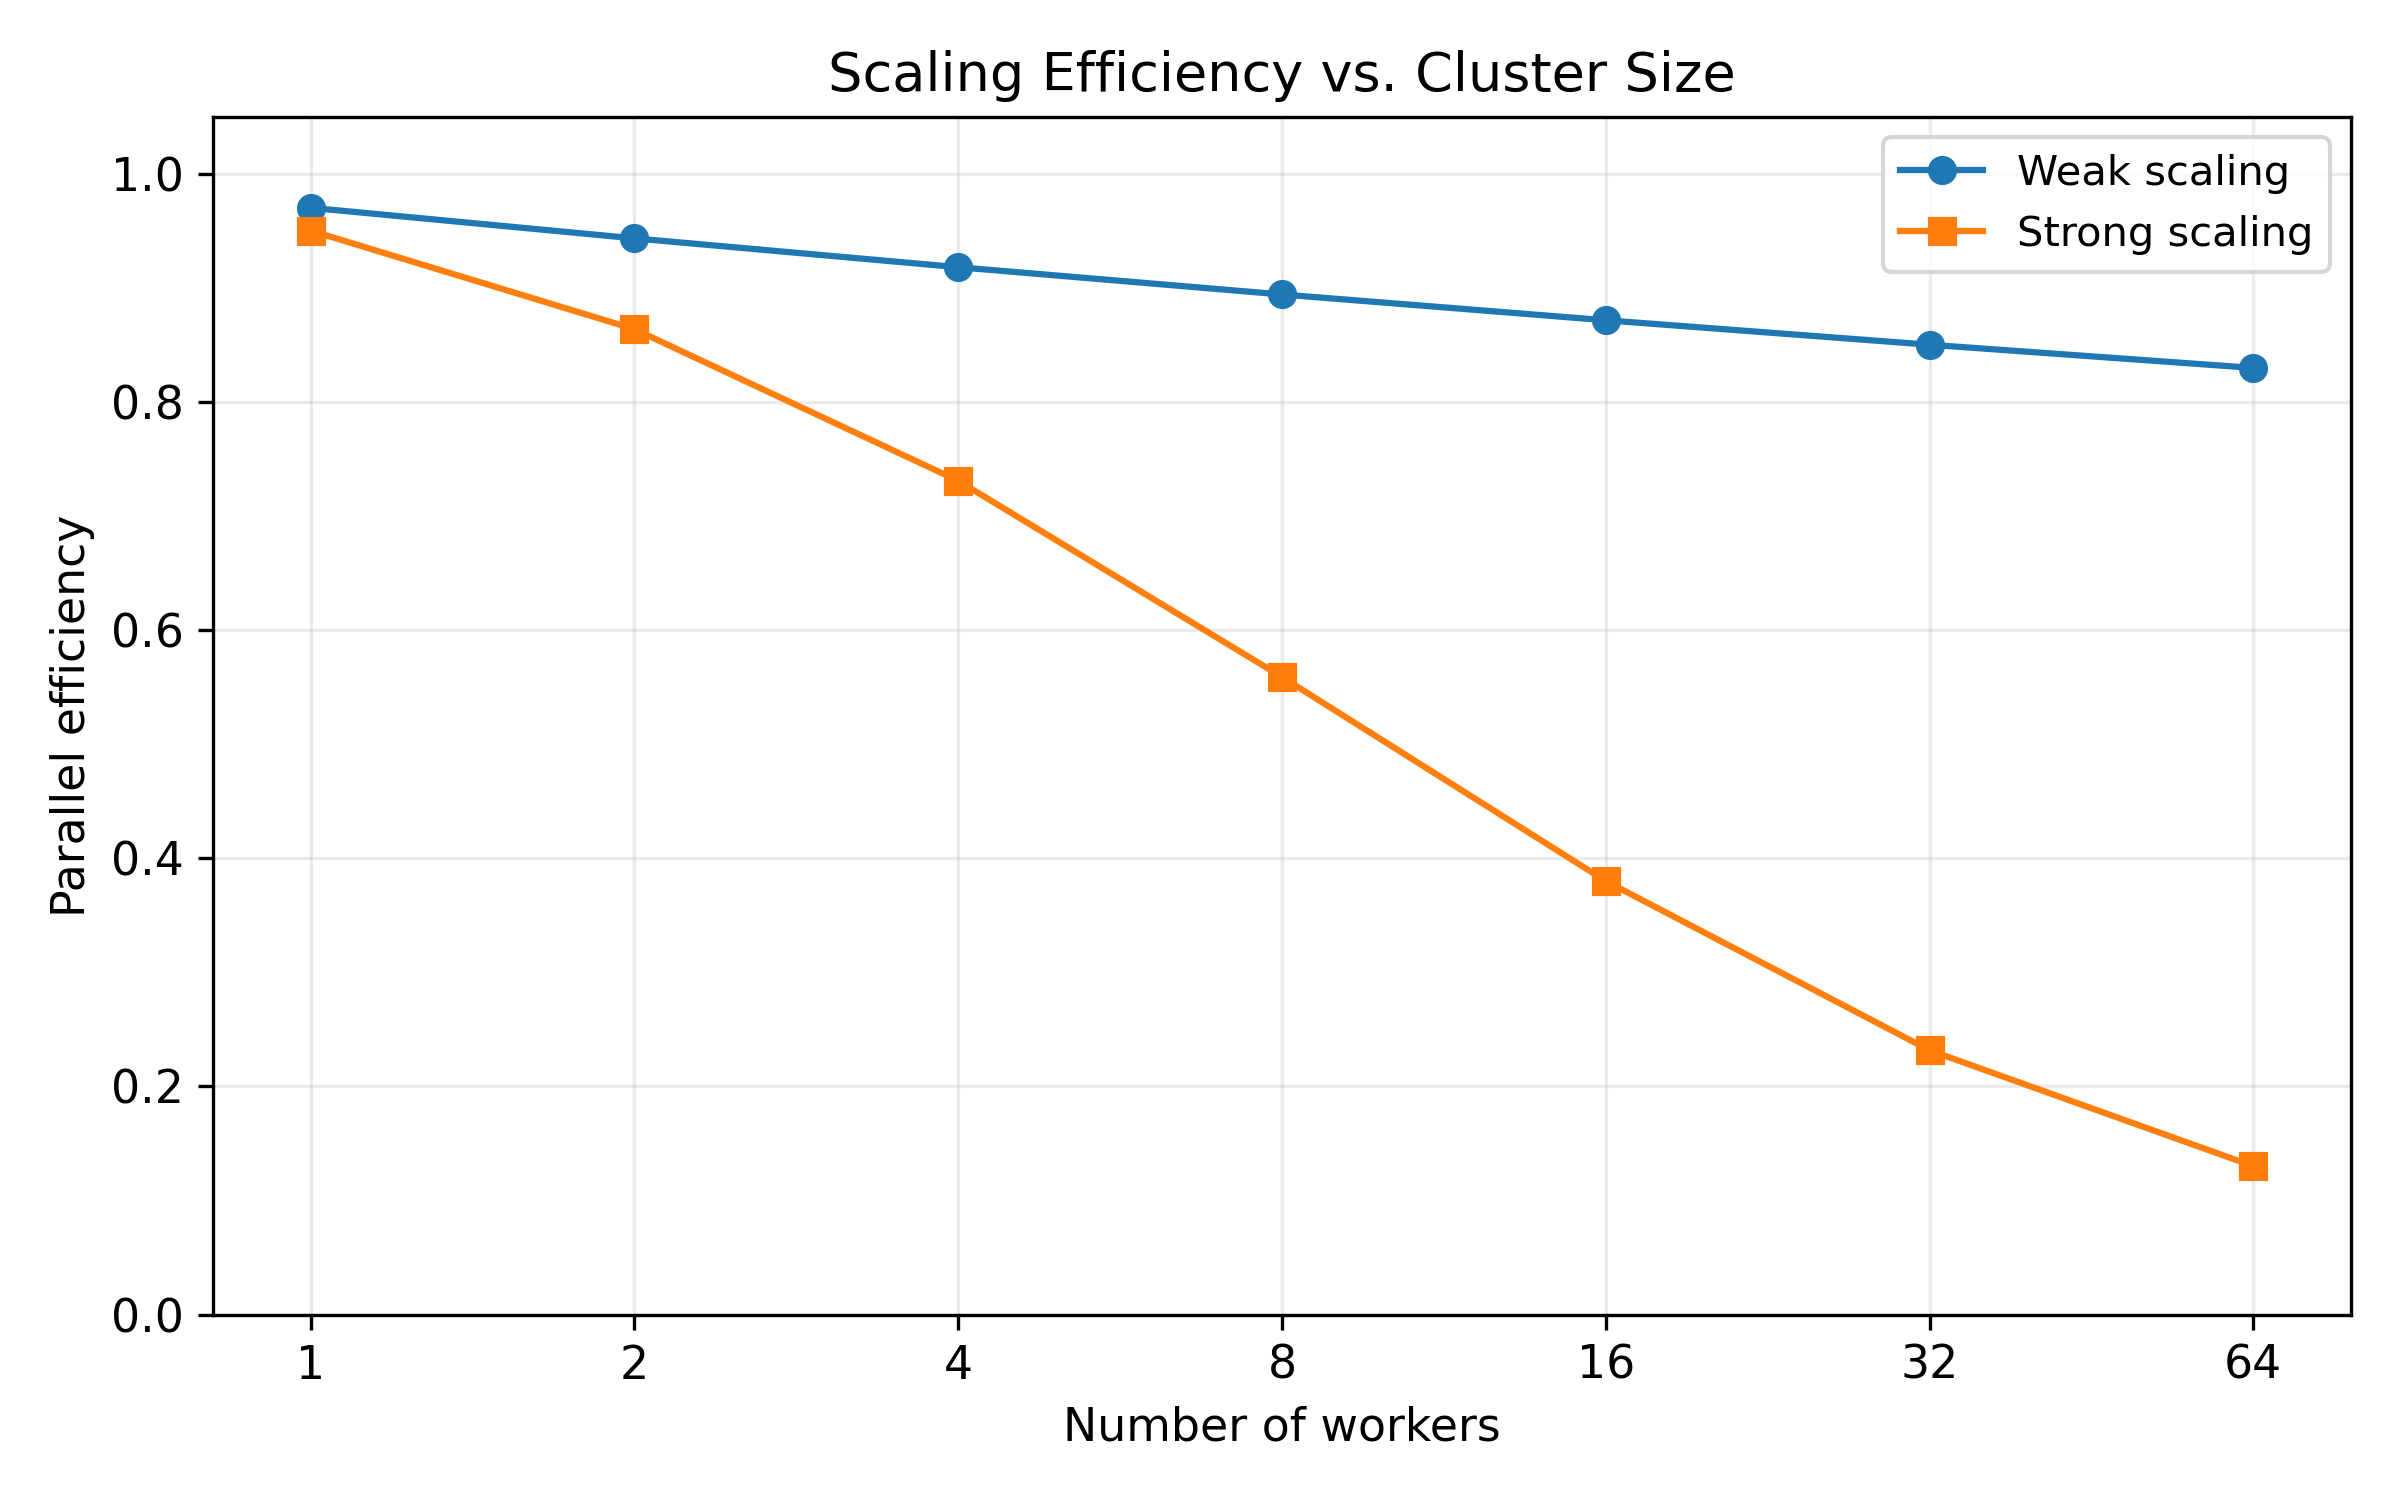
\includegraphics[width=0.85\textwidth]{scaling_efficiency.png}
  \caption{Scaling efficiency curves for weak and strong scaling experiments. Communication-optimized configurations maintain higher efficiency at large node counts.}
  \label{fig:scaling_efficiency}
\end{figure}
\FloatBarrier

\section*{Further Reading}
\begin{itemize}
  \item Priya Goyal et al. ``Accurate, Large Minibatch SGD: Training ImageNet in 1 Hour.'' 2017.
  \item Nitish S. Keskar et al. ``On Large-Batch Training for Deep Learning.'' ICLR 2017.
  \item Chen Ying et al. ``A Survey on Distributed Training of Deep Learning Models.'' 2022.
  \item Rich Caruana et al. ``Ensemble Selection from Libraries of Models.'' ICML 2004.
\end{itemize}

\end{document}
